\documentclass{beamer}
\usepackage[utf8]{inputenc}
\usepackage{ctex, hyperref}
\usepackage{wrapfig}
\graphicspath{ {imagens/} }

\author{エリキ後藤}
\title{折り紙 - Origami}
\subtitle{}
\institute{UNICAMP}
\date{5月}

\usetheme{Madrid}
\begin{document}

\kaishu
\begin{frame}
    \titlepage
\end{frame}

\section{じこしょうかい}
\begin{frame}{じこしょうかい}
    \begin{flushleft}
    \Huge
        はじめまして,
    \end{flushleft}
    \Large
    \begin{flushright}
        今日は折り紙についてはっぴょうします。
    \end{flushright}
\end{frame}

\section{折り紙は何ですか}
\begin{frame}{折り紙何ですか}

	\begin{wrapfigure}{r}{0.5\textwidth}
			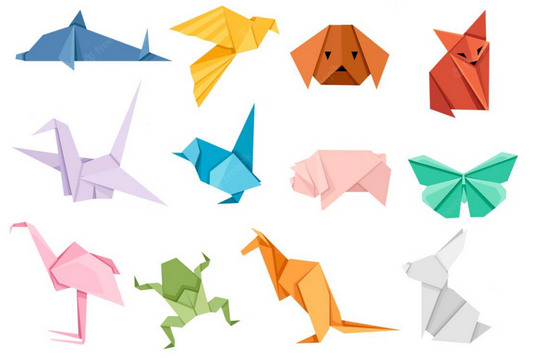
\includegraphics[width=0.5\textwidth]{a.png}
	\end{wrapfigure}
	でんとうてきには
	\begin{itemize}
		\item かみを切らないで、
		\item なにもはらないで、
		\item 四角のかみをつかいます。
	\end{itemize}
\end{frame}
\begin{frame}
	\begin{wrapfigure}{l}{0.5\textwidth}
			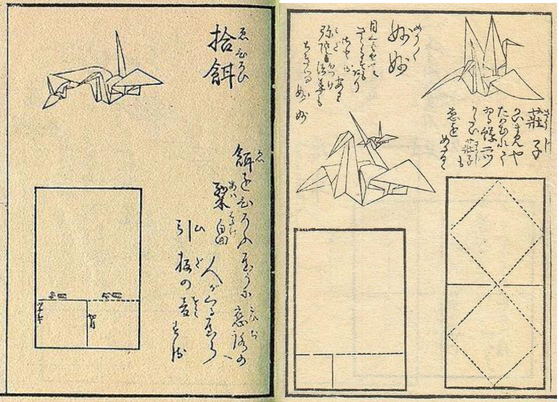
\includegraphics[width=0.5\textwidth]{aa.png}
	\end{wrapfigure}
	むかし。。。
	\begin{itemize}
		\item かみは高っかた、
		\item 折り紙は口頭でおしえられました、
		\item 一千 七百九十七年: ひでんせんばづるおりかた。
	\end{itemize}、
\end{frame}
\section{Origami no Japão}

\section{現在}
\begin{frame}{現在}
	\begin{wrapfigure}{l}{0.5\textwidth}
			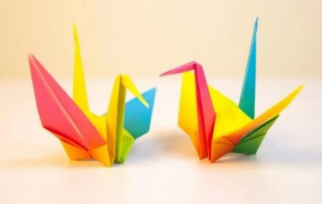
\includegraphics[width=0.5\textwidth]{aaa.png}
	\end{wrapfigure}
    日本で折り紙はとてもにんきあります。
    
    つるは
    \begin{itemize}
    	\item けんこうと
    	\item へいわと
    	\item しあわせをあらわします
    \end{itemize}
    
\end{frame}
\end{document}